\documentclass[12pt, letterpaper]{article}
\usepackage[utf8]{inputenc}
\usepackage{graphicx, amsfonts, amsmath, amsthm, amssymb}

\title{Autocorrelation in Temperature data from Key West}
\author{\\Jake Curry\\j.curry18@imperial.ac.uk}
\date{October 2018}

\begin{titlepage}
\maketitle
\end{titlepage}

\begin{document}
The results of the autocorrelation practical indicate that temperatures in a given year are dependent on the previous year - statistically significantly so. 

My estimated p-value is $3e-04$, as the correlation coefficient of the unjumbled years fell within the top 2.5 percent of all correlation coefficients found from ten thousand randomised samples - this means that the correlation found is not just random, or that it would've occured by chance at this level with a propability of $3e-04$. 

The below density plot (Figrue 1.) shows where the correlation coefficient found from the non-random sample falls in the continuum of correlation coefficients found from ten thousand randomised samples (which produce a near-normal distribution). 

\begin{figure}[h]
	{wrapfigure}{r}{0.25\textwidth}
\caption{Correlation coefficients of randomised temperature data year pairs, showing the non-random datas correlation coefficient}
\centering
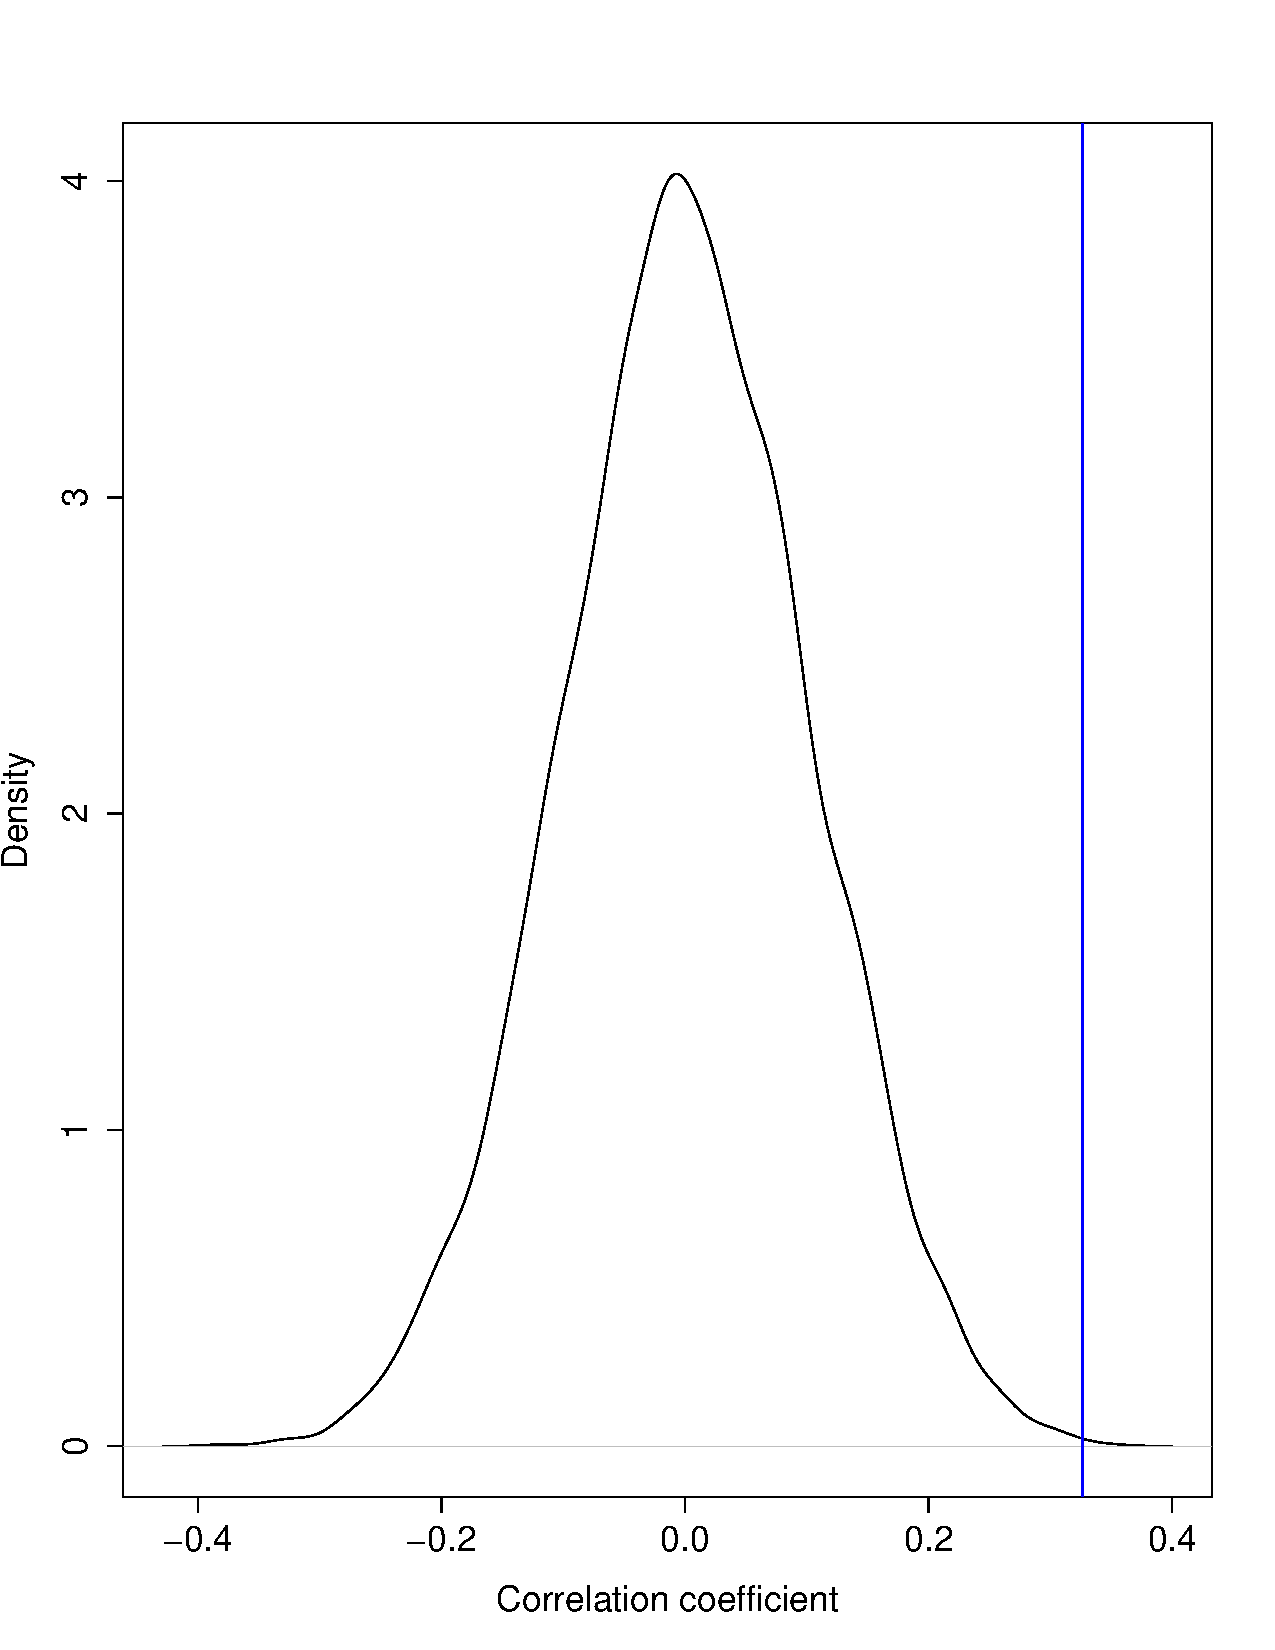
\includegraphics[width=12cm]{AutoCorrPlot}
\end{figure}

\end{document}
